\documentclass{report}
\title{\Large  Physics 20 - Encryption and Cryptography}
\author{\large Shubh Agrawal, \normalsize\emph{Class of 2022}}
\date{\small December 10, 2018}
\usepackage[a4paper,top=2cm, left=2.5cm,width=13cm,bottom=2cm,right=2.5cm]{geometry}
\usepackage{amsthm, amsmath, amssymb, tipa, graphicx, caption, subcaption, float, fancyhdr, graphics, verbatim}

\pagestyle{fancy}
\lhead{Shubh Agrawal}
\rhead{Physics 20}
\chead{Encryption}

\begin{document}
\maketitle
\section*{Threat Modeling}
MIT and Caltech have shared a inter-collegiate prank culture. At the 2005 pre-freshman weekend event, Caltech undergrads played several tricks on current and prospective students. MIT, in an attempt of retaliation, is now on campus in Pasadena with physical and wireless access to routers, on which information about Caltech's counter-measures to prevent such pranks is exchanged between students. The adversaries have access to the communication channels and can monitor network traffic; it is a classic example of a Man In The Middle (and a potential Denial of Service) attack.
\section*{Public Key Sharing - Diffie–Hellman key exchange}
The Diffie-Hellman (DH) public key exchange method, like several other encryption protocols, is based on the fact that factorization of large numbers using classical computers is computationally expensive. The protocol provides a secure method to generate a shared private key between two users which be used to inter-communicate information through an insecure channel. The two users first agree on two prime numbers $g$ and $p$, which can be made public, such that $p$ is computationally large and $g$ is a primitive root modulo $p$. Generally, $p$ is chosen such that $\frac{p-1}{2}$ is also prime, thus adding another computationally expensive layer to the protocol. Both users (say X and Y) choose a large random number as their keys, say $a$ and $b$ respectively. User X computes the value $A = g^a \mod p$, and User Y computes the value $B = g^b \mod p$; they share these two values ($A$ and $B$) through the public channel. The shared key $K$ is then computed as $K=B^a \mod p$ by User X and $K=A^b \mod p$ by User Y. Note that under the properties of this mathematical system, both expressions for $K$ give the same value $K=g^{ab}\mod p$. For a third potentially malicious user on the public communication channel, finding the values for $a$ and $b$ using the other public values is a discrete logarithmic problem, which is infeasible for large $p$. 

A probable vulnerability of this protocol is that an adversary can potentially perform a single enormous computation for a particular prime, and use that pre-computation to break any connection based on that prime. A counter-solution to the problem is using 2048-bit system keys for which pre-computation is impractical.

The chances of a man-in-the-middle attack are increased as the protocol does not verify the user with which the key negotiation is being carried out. A frequent counter is to use new session keys instead of long-term public keys.
\subsection*{Collision Attack}
The Python file \textit{DHkey.py}, which implements a basic version of the Diffie–Hellman protocol, also contains a brute-force ``classical collision attack'' which tries to find values of user X or/and user Y private keys which might give the same common key for the cryptographic hash, that is, the \textit{key()} function. The method runs through all possible permutations of the private keys [for the public pair $(p, g) = (23, 5)$] in the range of 10 to 500, and tries to find a pair of user private keys $(X, Y)$ for which the shared key $K$ is the same.
\section*{Crypto-program: gpg or GNU Privacy Guard}
I used a virtual machine running Ubuntu to test out the command line utility of the statements based on \textit{gpg}. A notable characteristic I saw, while using this module to generate random private/public keys, was how giving random input through the mouse or the keyboard (or even memory disks) increased the entropy and randomness of hexadecimals/alphanumeric strings generated; this can be an overall issue for a static isolated large-scale system. Also, the GNU protocol is generally, being a stand-alone cmd-based system, not very integrable or non-incorporated into other software.

The ``proof of action'' resides in two facts: I generated a random string, representing a secure key which expires in December 2020.
\begin{figure}[H]
	\centering
	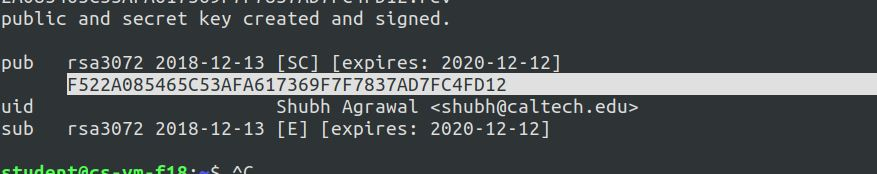
\includegraphics[width = 0.8\textwidth]{KEY.jpg}
	\label{key}
\end{figure}
Additionally, this file submission was/is encrypted by the same protocol/module.
\section*{Secure Authentication}
\begin{itemize}
	\item The channel of authentication must be secure and anonymous.
	\item The information required from the user should be simple to input and/or remember.
	\item Simultaneously, it must be difficult to decrypt or compromise, notably through a brute-force classical collision attack.
\end{itemize}
Common ways to compromise even strong passwords include phishing, or data breaches at consumer-faced servers.
\section*{Conclusion}
The introduction to how public channel key sharing works was a completely new topic to me; the idea of pre-computation as a threat in brute force or cipher collision attacks was interesting. 

The overall system of using the Diffie–Hellman protocol to obtain a shared key, along with using gpg protocol for encryption of information over the shared (wireless) channel is sufficiently robust to address the threat of MIT pranks (or Caltech pranks being leaked).
\end{document}